
Because the precision of the \efield measurement relies heavily on a precise knowledge of the laser beam tracks, an independent measurement of their direction for some specific positions is required. The \dlong{lbls} (\dshort{lbls}) addresses this requirement. 
While the direction of the laser beam will be very well known based on the reading from the encoders on the laser beam steering mechanism,  residual uncertainty or unpredictable shift in the pointing direction will remain. 
Keeping in mind the long length of the ionization track of more than \SI{12}{\m}, even a small offset in the pointing direction can lead to vastly different ionization track locations, especially close to the end of the track. Such inaccuracies will directly affect our ability to precisely calibrate any variations in the \efield.

\subsubsection{Design}
The \dword{lbls} is designed to address the problem of precise and accurate knowledge of the laser track coordinates. 
Two complementary systems are planned, one based on PIN diodes and another based on mirrors.

\paragraph{PIN diode system for laser beam location}
The design for the system using PIN diodes is based on the existing system that was built for the mini\dword{captain} experiment~\cite{Berns:2013usa}.

The \dword{lbls} consists of groups of \num{9} PIN diodes, operating in passive, photovoltaic mode. These are GaP diodes with a sensitivity range extending down to  \SI{200}{\nano\m} wavelength; thus, detecting \SI{266}{\nano\m} light is straightforward. %Figure~\ref{fig:GaP_diode_room_temp} shows signal detected at room and cryogenic temperatures. The PIN diode is illuminated by the \SI{266}{\nano\m} light from the Nd:Yag laser in the laboratory set at lowest possible setting for minimal power. 
PIN diodes are placed at the bottom of the cryostat and receive direct laser light\footnote{This is a difference with respect to the miniCAPTAIN system, that does not observe direct light, but detects fluorescence in the \frfour.} passing through the cathode and ground grids. Drawings of one such group of PIN diodes are shown in Figure~\ref{fig:GaP_assembly}. With the group of \num{9} photodiodes, we can detect not only the beam but also crudely characterize its profile, giving a more precise location of the central beam pulse axis. 

\begin{dunefigure}[Cluster assembly of the miniCAPTAIN \dshort{lbls}]{fig:GaP_assembly}
{(Left) \dword{lbls} cluster mounted on the opposite wall from the laser periscope to detect and accurately determine the end point of the laser beam. (Right)
Profile of the \dword{lbls} group mounted on the PCB. GaP diodes come with pins that use pair of twisted wires to transport the signal.}
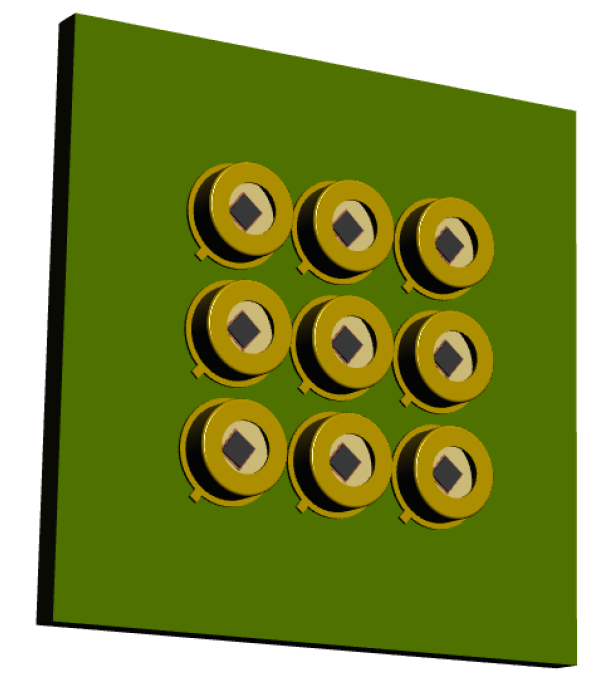
\includegraphics[width=0.35\linewidth]{GaP_assembly.png} 
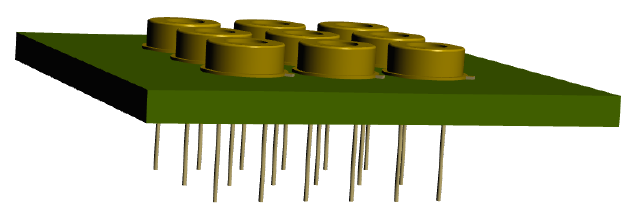
\includegraphics[width=0.45\linewidth]{GaP_assembly_profile.png} 
\end{dunefigure}

The exact number of pads is still under discussion, but as a minimum they should be such that each laser has at least two pads within a reachable range, i.e, within \SI{20}{\m} (this leads to a minimum of 10 pads). The locations of the pads will be carefully surveyed after installation and prior to closing of the cryostat. The laser should always send the first pulse in the direction of the \dword{lbls} before proceeding into a calibration sequence. In this way, the absolute location of the initial laser track will be determined with high accuracy. The location of the other laser tracks will also be determined with high accuracy with respect to the initial track thanks to the high precision of the rotary encoders.



\paragraph{Mirror-based beam positioning system:}

In addition to the PIN diode system, we will also have clusters of small mirrors that allow measuring the beam end position using its reflections.

Figure~\ref{fig:laser_mirror_positioning} shows a conceptual sketch with a cluster of \num{6} mirrors located close to each other, but with different angles. 
When the beam hits one of the mirrors, it will be reflected back into the \dword{tpc}, and the reflection angle unambiguously identifies which mirror was actually hit. 

With small mirrors, \SI{5}{\milli\m} in diameter, the required positioning precision would be met if these mirrors are placed at distances further than \SI{10}{\m}. The preferred location is, therefore, on the opposite \dword{fc} side wall. Because the top half of the \dword{fc} will be covered with \dword{pds} reflector panels, only lower half of the \dword{fc} profiles can be used. For redundancy, each laser periscope should have two associated mirror clusters. 

The simplest solution would be to have the reflecting surface made of polished aluminum, so the cluster could be a single block. Tests of the actual reflectivity of the (oxidized) surface will be part of the development plan. An alternative would be small dielectric mirrors.

\begin{dunefigure}[Mirror-based laser beam positioning system]{fig:laser_mirror_positioning}
{View of the mirror cluster for the beam positioning system inserted in the \dword{fc} profiles~\cite{bib:yu2019a}.}
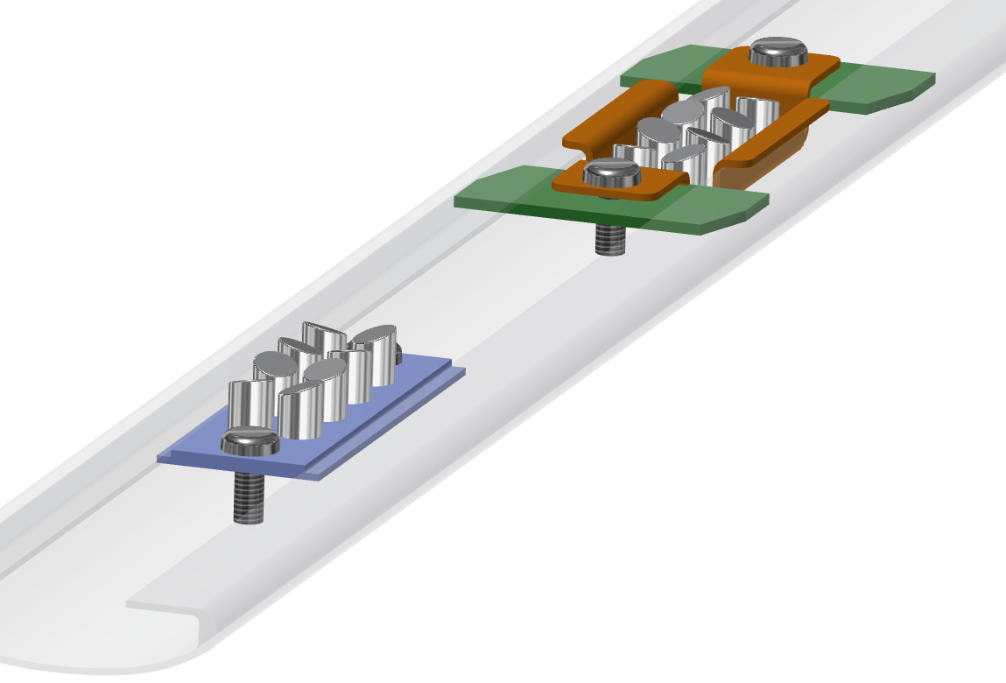
\includegraphics[width=0.7\linewidth]{laser_mirror_positioning.pdf}
\end{dunefigure}

\subsubsection{Development plan}

Further optimization of the PIN diode %\dword{lbls} 
 assembly to reduce electronic noise and cross-talk is required. Also, the size and shape of the cluster that would best collect the light coming through the field cage gaps needs to be optimized.  Another important aspect is durability of the system that will require extensive running in the cryogenic conditions with  a large number of cool-downs to validate GaP for extended use in DUNE. Finally, alternatives to GaP diodes such as SiPMs are under consideration. While SiPMs require power, their sensitivity to single photons makes them a desirable candidate for low light signals and more accurate beam direction reconstruction. 

As for the mirror-based system, the capability of the \dword{tpc} to identify the reflected beam will depend on how diffuse the reflectivity on the aluminum surfaces will be. A full test must be carried out at \dword{pdsp}, including alternative options such as using mirrors. Small dielectric mirrors for \SI{266}{\nano\m} with \SI{6.35}{\milli\m} diameter are commercially available.

















